% !TEX program = xelatex
% =========================================================
%  中英对照版入口 -- pdf-to-chinese-latex skill
%
%  本文件不含正文。它在加载 main.tex 之前定义一套“对照版”宏，
%  于是同一份 main.tex 编译出两个版本：
%     xelatex main.tex            -> main.pdf            纯中文译文
%     xelatex main_bilingual.tex  -> main_bilingual.pdf  上原文、下译文
%  main.tex 里用 \providecommand 定义的是纯中文版宏；因为这里先定义，
%  那些 \providecommand 不会覆盖这里的版本。
%
%  宏一览（正文写法见 SKILL.md Step 5）：
%     \bipar{原文段落}{中文段落}          正文段落（含摘要、公式前后的段落片段）
%     \bisection{原文}{中文}              编号章节标题（另有 \bisubsection / \bisubsubsection）
%     \bihead{原文}{中文}                 短标题：论文标题、表/算法标题、\section* 标题
%     \biitem{原文}{中文}                 列表项（代替 \item）
%     \bifoot{原文}{中文}                 脚注（代替 \footnote；只写在中文那一半里）
%     \bithanks{原文}{中文}               标题区作者脚注（代替 \thanks）
%  “摘要”“参考文献”两个标题由本文件自动配上 Abstract / References。
%
%  Overleaf：Menu -> Main document 选 main_bilingual.tex 即可编译对照版。
%  不要在本文件里写正文——正文只在 main.tex 里维护一份。
% =========================================================

% 原文一侧的颜色（深灰），与中文译文区分
\DeclareRobustCommand{\bisrcstyle}{\color[gray]{0.35}}

% 段落：原文一段、译文一段，两段都不缩进、尽量不分页拆开，每组之间留空
\newcommand{\bipar}[2]{\par\addvspace{0.7em}{\noindent\bisrcstyle #1\par}\nopagebreak\noindent #2}

% 短标题：原文一行（灰）、译文一行；PDF 书签只用中文
\DeclareRobustCommand{\bihead}[2]{\texorpdfstring{{\bisrcstyle #1}\\*#2}{#2}}

% 编号章节：页眉 / 目录 / 书签只用中文，正文标题上原文下中文
\newcommand{\bisection}[2]{\section[#2]{{\bisrcstyle #1}\\*#2}}
\newcommand{\bisubsection}[2]{\subsection[#2]{{\bisrcstyle #1}\\*#2}}
\newcommand{\bisubsubsection}[2]{\subsubsection[#2]{{\bisrcstyle #1}\\*#2}}

% 列表项与脚注
\newcommand{\biitem}[2]{\item{\bisrcstyle #1\par}\nopagebreak #2}
\newcommand{\bifoot}[2]{\footnote{{\bisrcstyle #1}\par #2}}
\newcommand{\bithanks}[2]{\thanks{{\bisrcstyle #1}\par #2}}

\makeatletter
\AddToHook{begindocument/end}{%
  % “摘要”“参考文献”标题配原文；页眉仍只用中文
  \let\bi@zhabstractname\abstractname
  \let\bi@zhrefname\refname
  \renewcommand{\abstractname}{{\bisrcstyle Abstract}\\*\bi@zhabstractname}%
  \renewcommand{\refname}{{\bisrcstyle References}\\*\bi@zhrefname}%
  % 对照版正文约为译文版两倍长，放宽浮动体参数，减少只放一张图的半空页
  \renewcommand{\topfraction}{0.9}%
  \renewcommand{\bottomfraction}{0.8}%
  \renewcommand{\textfraction}{0.07}%
  \renewcommand{\floatpagefraction}{0.8}%
  \setcounter{topnumber}{3}%
  \setcounter{totalnumber}{4}%
}
\def\bi@refmarks#1#2{\markboth{\bi@zhrefname}{\bi@zhrefname}}
\AddToHook{env/thebibliography/begin}{\let\@mkboth\bi@refmarks}
\makeatother

% !TEX program = xelatex
% =========================================================
%  Mistral 7B —— 中文译稿（pdf-to-chinese-latex skill）
%
%  原文：Albert Q. Jiang et al., "Mistral 7B", arXiv:2310.06825v1 [cs.CL], 2023.
%  原文以 CC BY 4.0 许可发布。
%
%  编译：XeLaTeX（Overleaf: Menu -> Compiler -> XeLaTeX）。
%    xelatex main.tex            -> main.pdf            纯中文译文
%    xelatex main_bilingual.tex  -> main_bilingual.pdf  中英对照（上原文、下译文）
%  正文只在本文件维护；每个段落 / 标题 / 列表项 / 脚注都写成 原文–中文 一对。
% =========================================================
\documentclass[a4paper,11pt]{article}

\usepackage[UTF8,heading=true]{ctex}
\usepackage[a4paper,margin=2.5cm]{geometry}
\usepackage{amsmath,amssymb,amsthm}
\usepackage{graphicx}
\usepackage{booktabs}
\usepackage{array}
\usepackage{longtable}
\usepackage{caption}
\usepackage{enumitem}
\usepackage{algorithm}
\usepackage{algpseudocode}
\usepackage{xcolor}
\usepackage[hidelinks,colorlinks=false]{hyperref}
\usepackage{url}
\usepackage{tabularx}
\usepackage{multirow}
\usepackage{float}
\usepackage{flafter}     % 浮动体不出现在其引用位置之前（避免表格跑到章节标题上方）

\graphicspath{{images/}}
\captionsetup{font=small,labelfont=bf}
\setlength{\parskip}{0.4em}
\setlength{\emergencystretch}{2em} % 中英混排时减少行溢出
% 英文短横线 – (U+2013) 按西文字符排版（xeCJK 默认把它当作中文标点，用宋体并吞掉其后的空格）
\xeCJKDeclareCharClass{Default}{"2013}
% 放宽浮动体参数，减少只放一两个浮动体的半空页
\renewcommand{\topfraction}{0.9}
\renewcommand{\bottomfraction}{0.8}
\renewcommand{\textfraction}{0.07}
\renewcommand{\floatpagefraction}{0.8}
\setcounter{topnumber}{3}
\setcounter{totalnumber}{4}

% --- 中英对照宏（纯中文版定义；main_bilingual.tex 会预先定义对照版）---
\providecommand{\bipar}[2]{#2}
\providecommand{\bihead}[2]{#2}
\providecommand{\bisection}[2]{\section{#2}}
\providecommand{\bisubsection}[2]{\subsection{#2}}
\providecommand{\bisubsubsection}[2]{\subsubsection{#2}}
\providecommand{\biitem}[2]{\item #2}
\providecommand{\bifoot}[2]{\footnote{#2}}
\providecommand{\bithanks}[2]{\thanks{#2}}
% -------------------------------------------------------------------------

\title{\bfseries Mistral 7B}
\author{\small\bfseries
Albert Q. Jiang, Alexandre Sablayrolles, Arthur Mensch, Chris Bamford,\\
\small\bfseries Devendra Singh Chaplot, Diego de las Casas, Florian Bressand, Gianna Lengyel,\\
\small\bfseries Guillaume Lample, Lucile Saulnier, Lélio Renard Lavaud, Marie-Anne Lachaux,\\
\small\bfseries Pierre Stock, Teven Le Scao, Thibaut Lavril, Thomas Wang, Timothée Lacroix,\\
\small\bfseries William El Sayed\\[10pt]

\includegraphics[width=0.42\textwidth]{logo.png}}
\date{\small 原文发布于 arXiv（arXiv:2310.06825v1 [cs.CL]），2023 年 10 月 10 日\\
\small \href{https://arxiv.org/abs/2310.06825}{\texttt{https://arxiv.org/abs/2310.06825}}\quad 原文许可：CC BY 4.0}

\begin{document}
\maketitle

\begin{abstract}
\bipar{We introduce Mistral 7B, a 7–billion-parameter language model engineered for superior performance and efficiency. Mistral 7B outperforms the best open 13B model (Llama 2) across all evaluated benchmarks, and the best released 34B model (Llama 1) in reasoning, mathematics, and code generation. Our model leverages grouped-query attention (GQA) for faster inference, coupled with sliding window attention (SWA) to effectively handle sequences of arbitrary length with a reduced inference cost. We also provide a model fine-tuned to follow instructions, Mistral 7B – Instruct, that surpasses Llama 2 13B – chat model both on human and automated benchmarks. Our models are released under the Apache 2.0 license.}{\noindent 我们推出 Mistral 7B——一个为兼顾卓越性能与高效率而设计的 70 亿参数语言模型。Mistral 7B 在所有评测基准（benchmark）上均优于目前最好的开放 13B 模型（Llama 2）；在推理（reasoning）、数学和代码生成方面，它还优于已发布的最佳 34B 模型（Llama 1）。我们的模型利用分组查询注意力（grouped-query attention, GQA）来加快推理（inference）速度，并结合滑动窗口注意力（sliding window attention, SWA），以更低的推理成本有效处理任意长度的序列。我们还提供了一个经过微调（fine-tuning）以遵循指令的模型 Mistral 7B – Instruct，它在人工评测和自动化评测基准上均超过了 Llama 2 13B – Chat 模型。我们的模型以 Apache 2.0 许可证发布。}

\bipar{\textbf{Code:} \url{https://github.com/mistralai/mistral-src}\\
\textbf{Webpage:} \url{https://mistral.ai/news/announcing-mistral-7b/}}{\noindent\textbf{代码：}\url{https://github.com/mistralai/mistral-src}\\
\textbf{网页：}\url{https://mistral.ai/news/announcing-mistral-7b/}}
\end{abstract}

% =========================================================
\bisection{Introduction}{引言}
\label{sec:intro}

\bipar{In the rapidly evolving domain of Natural Language Processing (NLP), the race towards higher model performance often necessitates an escalation in model size. However, this scaling tends to increase computational costs and inference latency, thereby raising barriers to deployment in practical, real-world scenarios. In this context, the search for balanced models delivering both high-level performance and efficiency becomes critically essential. Our model, Mistral 7B, demonstrates that a carefully designed language model can deliver high performance while maintaining an efficient inference. Mistral 7B outperforms the previous best 13B model (Llama 2, \cite{ref26}) across all tested benchmarks, and surpasses the best 34B model (LLaMa 34B, \cite{ref25}) in mathematics and code generation. Furthermore, Mistral 7B approaches the coding performance of Code-Llama 7B \cite{ref20}, without sacrificing performance on non-code related benchmarks.}{在快速发展的自然语言处理（Natural Language Processing, NLP）领域，对更高模型性能的追逐往往需要不断扩大模型规模。然而，这种规模扩展（scaling）通常会增加计算成本和推理延迟（inference latency），从而抬高在实际应用场景中部署模型的门槛。在此背景下，寻找既能提供高水平性能、又兼具效率的均衡模型变得至关重要。我们的模型 Mistral 7B 表明，经过精心设计的语言模型能够在保持高效推理的同时提供高性能。Mistral 7B 在所有测试基准上均优于此前最好的 13B 模型（Llama 2~\cite{ref26}），并在数学和代码生成方面超越了最好的 34B 模型（LLaMa 34B~\cite{ref25}）。此外，Mistral 7B 的代码能力接近 Code-Llama 7B~\cite{ref20}，同时并未牺牲在非代码类基准上的性能。}

\bipar{Mistral 7B leverages grouped-query attention (GQA) \cite{ref1}, and sliding window attention (SWA) \cite{ref6,ref3}. GQA significantly accelerates the inference speed, and also reduces the memory requirement during decoding, allowing for higher batch sizes hence higher throughput, a crucial factor for real-time applications. In addition, SWA is designed to handle longer sequences more effectively at a reduced computational cost, thereby alleviating a common limitation in LLMs. These attention mechanisms collectively contribute to the enhanced performance and efficiency of Mistral 7B.}{Mistral 7B 采用了分组查询注意力（grouped-query attention, GQA）\cite{ref1} 和滑动窗口注意力（sliding window attention, SWA）\cite{ref6,ref3}。GQA 显著加快了推理速度，同时降低了解码（decoding）阶段的内存需求，从而支持更大的批大小（batch size），进而获得更高的吞吐量（throughput）——这对实时应用而言是至关重要的因素。此外，SWA 旨在以更低的计算成本更有效地处理更长的序列，从而缓解了大语言模型（large language models, LLMs）的一个常见局限。这些注意力机制共同提升了 Mistral 7B 的性能与效率。}

\bipar{Mistral 7B is released under the Apache 2.0 license. This release is accompanied by a reference implementation facilitating easy deployment either locally or on cloud platforms such as AWS, GCP, or Azure using the vLLM \cite{ref17} inference server and SkyPilot. Integration with Hugging Face is also streamlined for easier integration. Moreover, Mistral 7B is crafted for ease of fine-tuning across a myriad of tasks. As a demonstration of its adaptability and superior performance, we present a chat model fine-tuned from Mistral 7B that significantly outperforms the Llama 2 13B – Chat model.}{Mistral 7B 以 Apache 2.0 许可证发布。随本次发布一同提供的还有一份参考实现（reference implementation）\footnote{\url{https://github.com/mistralai/mistral-src}}，借助 vLLM~\cite{ref17} 推理服务器（inference server）和 SkyPilot\footnote{\url{https://github.com/skypilot-org/skypilot}}，即可方便地在本地或 AWS、GCP、Azure 等云平台上完成部署。与 Hugging Face\footnote{\url{https://huggingface.co/mistralai}} 的集成也已得到简化，使用更加便捷。此外，Mistral 7B 的设计便于在各类任务上进行微调。为展示其适应性与卓越性能，我们给出了一个基于 Mistral 7B 微调得到的对话模型（chat model），其性能显著优于 Llama 2 13B – Chat 模型。}

\bipar{Mistral 7B takes a significant step in balancing the goals of getting high performance while keeping large language models efficient. Through our work, our aim is to help the community create more affordable, efficient, and high-performing language models that can be used in a wide range of real-world applications.}{在兼顾“高性能”与“大语言模型的高效率”这两个目标上，Mistral 7B 迈出了重要一步。我们希望通过这项工作，帮助社区打造更经济、更高效、性能更强的语言模型，使其能够应用于广泛的现实场景。}

% =========================================================
\bisection{Architectural details}{架构细节}
\label{sec:arch}

\begin{figure}[!htbp]
\centering
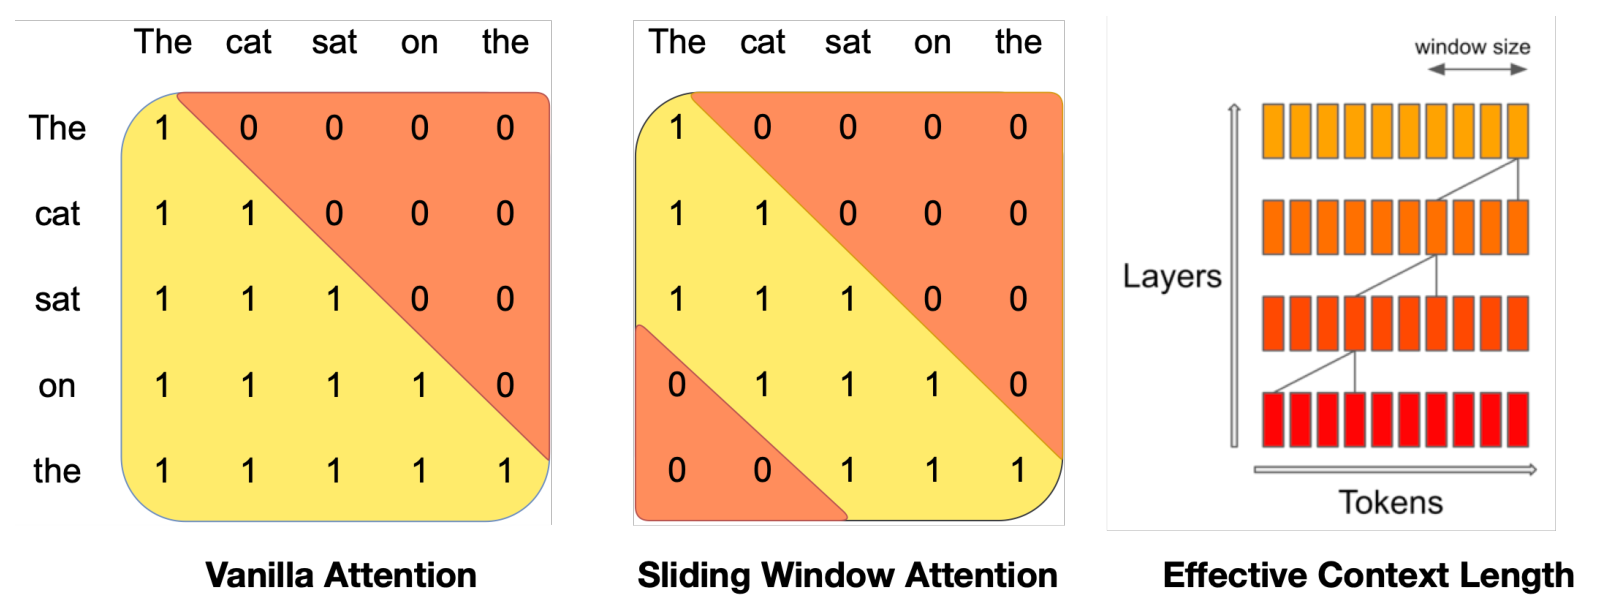
\includegraphics[width=0.85\textwidth]{fig1.png}
\caption{\bihead{\textbf{Sliding Window Attention.} The number of operations in vanilla attention is quadratic in the sequence length, and the memory increases linearly with the number of tokens. At inference time, this incurs higher latency and smaller throughput due to reduced cache availability. To alleviate this issue, we use sliding window attention: each token can attend to at most $W$ tokens from the previous layer (here, $W = 3$). Note that tokens outside the sliding window still influence next word prediction. At each attention layer, information can move forward by $W$ tokens. Hence, after $k$ attention layers, information can move forward by up to $k \times W$ tokens.}{\textbf{滑动窗口注意力。}普通注意力（vanilla attention）的运算量随序列长度呈二次方增长，内存占用则随词元（token）数量线性增长。在推理阶段，由于可用缓存减少，这会带来更高的延迟和更低的吞吐量。为缓解这一问题，我们采用滑动窗口注意力：每个词元最多只能关注（attend to）上一层中的 $W$ 个词元（图中 $W=3$）。注意，滑动窗口之外的词元仍会影响下一个词的预测。在每个注意力层，信息可以向前传递 $W$ 个词元；因此经过 $k$ 个注意力层后，信息最多可以向前传递 $k\times W$ 个词元。\\
\textbf{图中文字：}Vanilla Attention＝普通注意力；Sliding Window Attention＝滑动窗口注意力；Effective Context Length＝有效上下文长度；Layers＝层；Tokens＝词元；window size＝窗口大小。左、中两幅矩阵的行与列均为示例句“The cat sat on the”（那只猫坐在……上）中的词元，1 表示该位置可被关注，0 表示被屏蔽。}}
\label{fig:f1}
\end{figure}

\bipar{Mistral 7B is based on a transformer architecture \cite{ref27}. The main parameters of the architecture are summarized in Table~\ref{tab:t1}. Compared to Llama, it introduces a few changes that we summarize below.}{Mistral 7B 基于 Transformer 架构~\cite{ref27}，其主要架构参数汇总于表~\ref{tab:t1}。与 Llama 相比，它引入了若干改动，概述如下。}

\begin{table}[!htbp]
\centering
\caption{\bihead{\textbf{Model architecture.}}{\textbf{模型架构。}}}
\label{tab:t1}
\begin{tabular}{lr}
\toprule
参数 & 取值 \\
\midrule
\texttt{dim}         & 4096 \\
\texttt{n\_layers}    & 32 \\
\texttt{head\_dim}    & 128 \\
\texttt{hidden\_dim}  & 14336 \\
\texttt{n\_heads}     & 32 \\
\texttt{n\_kv\_heads} & 8 \\
\texttt{window\_size} & 4096 \\
\texttt{context\_len} & 8192 \\
\texttt{vocab\_size}  & 32000 \\
\bottomrule
\end{tabular}
\end{table}

\bipar{\textbf{Sliding Window Attention.} SWA exploits the stacked layers of a transformer to attend information beyond the window size $W$. The hidden state in position $i$ of the layer $k$, $h_i$, attends to all hidden states from the previous layer with positions between $i - W$ and $i$. Recursively, $h_i$ can access tokens from the input layer at a distance of up to $W \times k$ tokens, as illustrated in Figure~\ref{fig:f1}. At the last layer, using a window size of $W = 4096$, we have a theoretical attention span of approximately $131K$ tokens. In practice, for a sequence length of 16K and $W = 4096$, changes made to FlashAttention \cite{ref11} and xFormers \cite{ref18} yield a 2x speed improvement over a vanilla attention baseline.}{\textbf{滑动窗口注意力（Sliding Window Attention）。}SWA 利用 Transformer 的多层堆叠结构，使模型能够关注到窗口大小 $W$ 之外的信息。第 $k$ 层中位置 $i$ 处的隐藏状态（hidden state）$h_i$，会关注上一层中位置介于 $i-W$ 与 $i$ 之间的所有隐藏状态。以此递归，$h_i$ 最远可以访问输入层中与其相距 $W\times k$ 个词元（token）的信息，如图~\ref{fig:f1} 所示。在最后一层，若窗口大小取 $W=4096$，理论上的注意力跨度（attention span）约为 $131K$ 个词元。实践中，在序列长度为 16K、$W=4096$ 的条件下，对 FlashAttention~\cite{ref11} 和 xFormers~\cite{ref18} 所做的改动使速度比普通注意力基线（vanilla attention baseline）提升了 2 倍。}

\bipar{\textbf{Rolling Buffer Cache.} A fixed attention span means that we can limit our cache size using a rolling buffer cache. The cache has a fixed size of $W$, and the keys and values for the timestep $i$ are stored in position $i \bmod W$ of the cache. As a result, when the position $i$ is larger than $W$, past values in the cache are overwritten, and the size of the cache stops increasing. We provide an illustration in Figure~\ref{fig:f2} for $W = 3$. On a sequence length of 32k tokens, this reduces the cache memory usage by 8x, without impacting the model quality.}{\textbf{滚动缓冲区缓存（Rolling Buffer Cache）。}固定的注意力跨度意味着我们可以用滚动缓冲区缓存来限制缓存大小。缓存的大小固定为 $W$，时间步（timestep）$i$ 的键（key）和值（value）存放在缓存的第 $i \bmod W$ 个位置。因此，当位置 $i$ 大于 $W$ 时，缓存中过去的值会被覆盖，缓存大小也随之不再增长。图~\ref{fig:f2} 给出了 $W=3$ 时的示意\footnote{译者注：图~\ref{fig:f2} 的图注写作 $W=4$，与图中每行 4 个缓存位置一致；此处按原文照译。}。在长度为 32k 个词元的序列上，这一做法可将缓存的内存占用降至原来的八分之一，且不影响模型质量。}

\begin{figure}[!htbp]
\centering
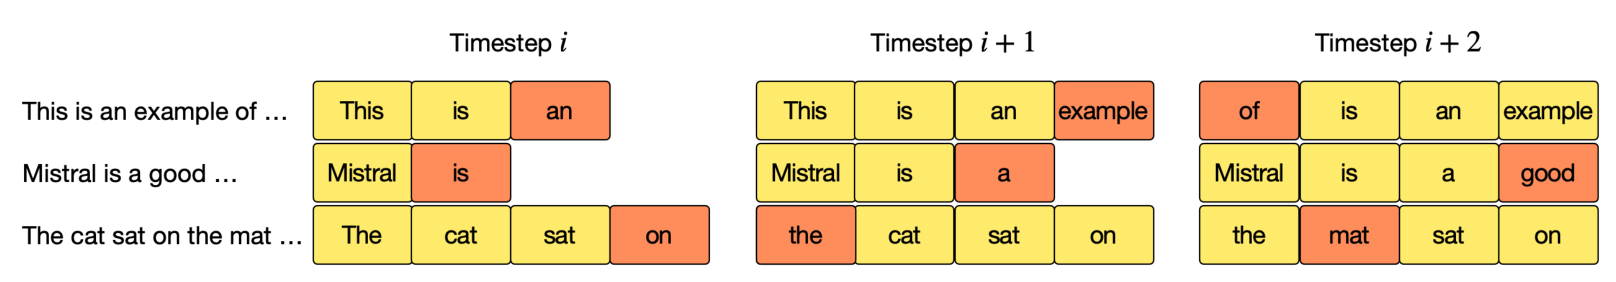
\includegraphics[width=0.85\textwidth]{fig2.png}
\caption{\bihead{\textbf{Rolling buffer cache.} The cache has a fixed size of $W = 4$. Keys and values for position $i$ are stored in position $i \bmod W$ of the cache. When the position $i$ is larger than $W$, past values in the cache are overwritten. The hidden state corresponding to the latest generated tokens are colored in orange.}{\textbf{滚动缓冲区缓存。}缓存的大小固定为 $W=4$。位置 $i$ 的键和值存放在缓存的第 $i \bmod W$ 个位置。当位置 $i$ 大于 $W$ 时，缓存中过去的值会被覆盖。最新生成的词元所对应的隐藏状态以橙色标出。\\
\textbf{图中文字：}Timestep $i$ / $i+1$ / $i+2$＝时间步 $i$ / $i+1$ / $i+2$。左侧三行是三条示例序列：“This is an example of …”（这是一个……的例子）、“Mistral is a good …”（Mistral 是一个好的……）、“The cat sat on the mat …”（那只猫坐在垫子上……）；每个方格代表缓存中的一个位置，格内为当前存放的词元。}}
\label{fig:f2}
\end{figure}

\bipar{\textbf{Pre-fill and Chunking.} When generating a sequence, we need to predict tokens one-by-one, as each token is conditioned on the previous ones. However, the prompt is known in advance, and we can pre-fill the $(k, v)$ cache with the prompt. If the prompt is very large, we can chunk it into smaller pieces, and pre-fill the cache with each chunk. For this purpose, we can select the window size as our chunk size. For each chunk, we thus need to compute the attention over the cache and over the chunk. Figure~\ref{fig:f3} shows how the attention mask works over both the cache and the chunk.}{\textbf{预填充与分块（Pre-fill and Chunking）。}生成序列时，由于每个词元都以它之前的词元为条件，我们需要逐个预测词元。然而，提示词（prompt）是事先已知的，因此可以用提示词预先填充（pre-fill）$(k, v)$ 缓存。如果提示词非常长，可以将其切分为更小的块（chunk），并逐块预填充缓存。为此，可以把窗口大小选作块的大小。于是，对于每个块，我们需要同时计算它在缓存上和在块内部的注意力。图~\ref{fig:f3} 展示了注意力掩码（attention mask）如何同时作用于缓存和当前块。}

\begin{figure}[!htbp]
\centering
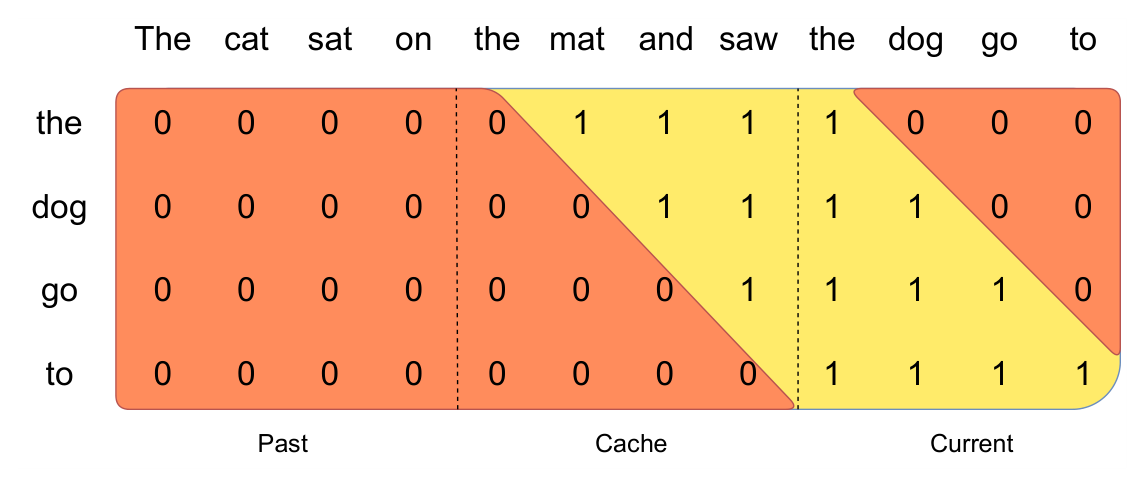
\includegraphics[width=0.75\textwidth]{fig3.png}
\caption{\bihead{\textbf{Pre-fill and chunking.} During pre-fill of the cache, long sequences are chunked to limit memory usage. We process a sequence in three chunks, ``The cat sat on'', ``the mat and saw'', ``the dog go to''. The figure shows what happens for the third chunk (``the dog go to''): it attends itself using a causal mask (rightmost block), attends the cache using a sliding window (center block), and does not attend to past tokens as they are outside of the sliding window (left block).}{\textbf{预填充与分块。}在预填充缓存时，长序列会被切分成块，以限制内存占用。我们把一个序列分成三块处理：“The cat sat on”“the mat and saw”“the dog go to”。图中展示的是第三块（“the dog go to”）的处理情况：它使用因果掩码（causal mask）关注自身（最右侧区块），使用滑动窗口关注缓存（中间区块），并且不关注更早的词元，因为它们位于滑动窗口之外（左侧区块）。\\
\textbf{图中文字：}Past＝过去的词元；Cache＝缓存；Current＝当前块。矩阵中 1 表示可被关注，0 表示被屏蔽。}}
\label{fig:f3}
\end{figure}

% =========================================================
\bisection{Results}{结果}
\label{sec:results}

\bipar{We compare Mistral 7B to Llama, and re-run all benchmarks with our own evaluation pipeline for fair comparison. We measure performance on a wide variety of tasks categorized as follow:}{我们将 Mistral 7B 与 Llama 进行比较，并且为保证比较的公平性，使用我们自己的评测流水线（evaluation pipeline）重新运行了全部基准测试。我们在多种任务上衡量模型性能，这些任务分类如下：}

\begin{itemize}
\biitem{\textbf{Commonsense Reasoning (0-shot):} Hellaswag \cite{ref28}, Winogrande \cite{ref21}, PIQA \cite{ref4}, SIQA \cite{ref22}, OpenbookQA \cite{ref19}, ARC-Easy, ARC-Challenge \cite{ref9}, CommonsenseQA \cite{ref24}}{\textbf{常识推理（Commonsense Reasoning；零样本，0-shot）：}Hellaswag~\cite{ref28}、Winogrande~\cite{ref21}、PIQA~\cite{ref4}、SIQA~\cite{ref22}、OpenbookQA~\cite{ref19}、ARC-Easy、ARC-Challenge~\cite{ref9}、CommonsenseQA~\cite{ref24}}
\biitem{\textbf{World Knowledge (5-shot):} NaturalQuestions \cite{ref16}, TriviaQA \cite{ref15}}{\textbf{世界知识（World Knowledge；5 样本，5-shot）：}NaturalQuestions~\cite{ref16}、TriviaQA~\cite{ref15}}
\biitem{\textbf{Reading Comprehension (0-shot):} BoolQ \cite{ref8}, QuAC \cite{ref7}}{\textbf{阅读理解（Reading Comprehension；零样本）：}BoolQ~\cite{ref8}、QuAC~\cite{ref7}}
\biitem{\textbf{Math:} GSM8K \cite{ref10} (8-shot) with maj@8 and MATH \cite{ref13} (4-shot) with maj@4}{\textbf{数学（Math）：}GSM8K~\cite{ref10}（8 样本，采用 maj@8，即对 8 次采样结果多数投票）和 MATH~\cite{ref13}（4 样本，采用 maj@4）}
\biitem{\textbf{Code:} Humaneval \cite{ref5} (0-shot) and MBPP \cite{ref2} (3-shot)}{\textbf{代码（Code）：}Humaneval~\cite{ref5}（零样本）和 MBPP~\cite{ref2}（3 样本）}
\biitem{\textbf{Popular aggregated results:} MMLU \cite{ref12} (5-shot), BBH \cite{ref23} (3-shot), and AGI Eval \cite{ref29} (3-5-shot, English multiple-choice questions only)}{\textbf{常用综合基准（Popular aggregated results）：}MMLU~\cite{ref12}（5 样本）、BBH~\cite{ref23}（3 样本）以及 AGI Eval~\cite{ref29}（3--5 样本，仅限英文多项选择题）}
\end{itemize}

\bipar{Detailed results for Mistral 7B, Llama 2 7B/13B, and Code-Llama 7B are reported in Table~\ref{tab:t2}. Figure~\ref{fig:f4} compares the performance of Mistral 7B with Llama 2 7B/13B, and Llama 1 34B in different categories. Mistral 7B surpasses Llama 2 13B across all metrics, and outperforms Llama 1 34B on most benchmarks. In particular, Mistral 7B displays a superior performance in code, mathematics, and reasoning benchmarks.}{Mistral 7B、Llama 2 7B/13B 和 Code-Llama 7B 的详细结果见表~\ref{tab:t2}。图~\ref{fig:f4} 按类别比较了 Mistral 7B 与 Llama 2 7B/13B 以及 Llama 1 34B\bifoot{Since Llama 2 34B was not open-sourced, we report results for Llama 1 34B.}{由于 Llama 2 34B 未开源，我们报告的是 Llama 1 34B 的结果。}的性能。Mistral 7B 在所有指标上均超过 Llama 2 13B，并在大多数基准上优于 Llama 1 34B。尤其是在代码、数学和推理基准上，Mistral 7B 表现出更为优越的性能。}

\begin{figure}[!htbp]
\centering
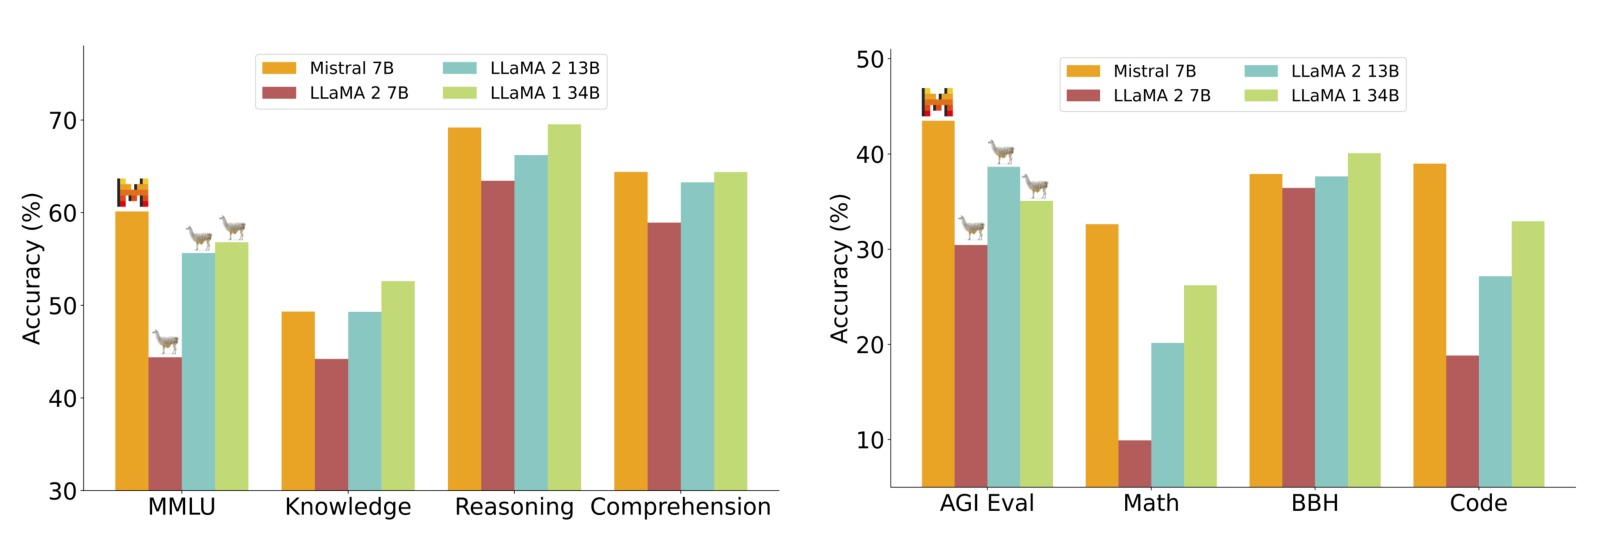
\includegraphics[width=0.85\textwidth]{fig4.png}
\caption{\bihead{\textbf{Performance of Mistral 7B and different Llama models on a wide range of benchmarks}. All models were re-evaluated on all metrics with our evaluation pipeline for accurate comparison. Mistral 7B significantly outperforms Llama 2 7B and Llama 2 13B on all benchmarks. It is also vastly superior to Llama 1 34B in mathematics, code generation, and reasoning benchmarks.}{\textbf{Mistral 7B 与不同 Llama 模型在多种基准上的性能。}为保证比较准确，所有模型的全部指标均使用我们的评测流水线重新评测。Mistral 7B 在所有基准上均显著优于 Llama 2 7B 和 Llama 2 13B；在数学、代码生成和推理基准上，它也大幅领先于 Llama 1 34B。\\
\textbf{图中文字：}纵轴 Accuracy (\%)＝准确率（\%）；横轴类别为 MMLU、Knowledge（知识）、Reasoning（推理）、Comprehension（理解）以及 AGI Eval、Math（数学）、BBH、Code（代码）；图例依次为 Mistral 7B、LLaMA 2 7B、LLaMA 2 13B、LLaMA 1 34B。}}
\label{fig:f4}
\end{figure}

\begin{table}[!htbp]
\centering
\caption{\bihead{\textbf{Comparison of Mistral 7B with Llama.} Mistral 7B outperforms Llama 2 13B on all metrics, and approaches the code performance of Code-Llama 7B without sacrificing performance on non-code benchmarks.}{\textbf{Mistral 7B 与 Llama 的比较。}Mistral 7B 在所有指标上均优于 Llama 2 13B，其代码性能接近 Code-Llama 7B，且没有牺牲非代码基准上的性能。}}
\label{tab:t2}
\footnotesize
\setlength{\tabcolsep}{2.4pt}
\resizebox{\textwidth}{!}{%
\begin{tabular}{llrrrrrrrrrrrr}
\toprule
模型 & 类型 & MMLU & HellaSwag & WinoG & PIQA & Arc-e & Arc-c & NQ & TriviaQA & HumanEval & MBPP & MATH & GSM8K \\
\midrule
LLaMA 2 7B  & 预训练 & 44.4\% & 77.1\% & 69.5\% & 77.9\% & 68.7\% & 43.2\% & 24.7\% & 63.8\% & 11.6\% & 26.1\% & 3.9\% & 16.0\% \\
LLaMA 2 13B & 预训练 & 55.6\% & \textbf{80.7\%} & 72.9\% & 80.8\% & 75.2\% & 48.8\% & \textbf{29.0\%} & \textbf{69.6\%} & 18.9\% & 35.4\% & 6.0\% & 34.3\% \\
\midrule
Code-Llama 7B & 微调 & 36.9\% & 62.9\% & 62.3\% & 72.8\% & 59.4\% & 34.5\% & 11.0\% & 34.9\% & \textbf{31.1\%} & \textbf{52.5\%} & 5.2\% & 20.8\% \\
\midrule
Mistral 7B & 预训练 & \textbf{60.1\%} & \textbf{81.3\%} & \textbf{75.3\%} & \textbf{83.0\%} & \textbf{80.0\%} & \textbf{55.5\%} & \textbf{28.8\%} & \textbf{69.9\%} & \textbf{30.5\%} & 47.5\% & \textbf{13.1\%} & \textbf{52.2\%} \\
\bottomrule
\end{tabular}}
\end{table}

\bipar{\textbf{Size and Efficiency.} We computed ``equivalent model sizes'' of the Llama 2 family, aiming to understand Mistral 7B models' efficiency in the cost-performance spectrum (see Figure~\ref{fig:f5}). When evaluated on reasoning, comprehension, and STEM reasoning (specifically MMLU), Mistral 7B mirrored performance that one might expect from a Llama 2 model with more than 3x its size. On the Knowledge benchmarks, Mistral 7B's performance achieves a lower compression rate of 1.9x, which is likely due to its limited parameter count that restricts the amount of knowledge it can store.}{\textbf{规模与效率（Size and Efficiency）。}我们计算了 Llama 2 系列的“等效模型规模”（equivalent model size），以了解 Mistral 7B 模型在成本—性能谱（cost-performance spectrum）中的效率（见图~\ref{fig:f5}）。在推理、理解和 STEM 推理（具体为 MMLU）上进行评测时，Mistral 7B 的表现相当于一个规模为其 3 倍以上的 Llama 2 模型所能达到的水平。在知识类基准上，Mistral 7B 的压缩率（compression rate）较低，为 1.9 倍，这很可能是因为其参数量有限，限制了它所能存储的知识量。}

\begin{figure}[!htbp]
\centering
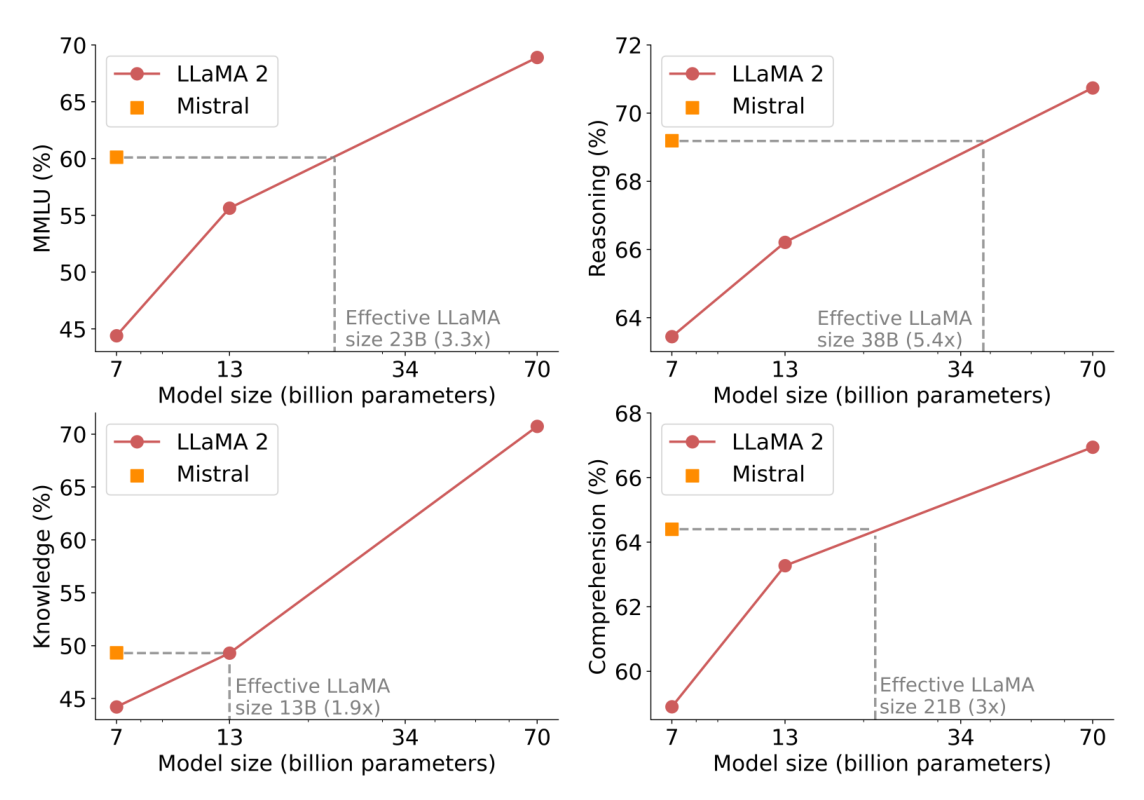
\includegraphics[width=0.65\textwidth]{fig5.png}
\caption{\bihead{\textbf{Results on MMLU, commonsense reasoning, world knowledge and reading comprehension for Mistral 7B and Llama 2 (7B/13B/70B)}. Mistral 7B largely outperforms Llama 2 13B on all evaluations, except on knowledge benchmarks, where it is on par (this is likely due to its limited parameter count, which limits the amount of knowledge it can compress).}{\textbf{Mistral 7B 与 Llama 2（7B/13B/70B）在 MMLU、常识推理、世界知识和阅读理解上的结果。}除在知识类基准上与 Llama 2 13B 持平外，Mistral 7B 在其余所有评测中都大幅优于 Llama 2 13B（持平很可能是因为其参数量有限，限制了它所能压缩的知识量）。\\
\textbf{图中文字：}横轴 Model size (billion parameters)＝模型规模（十亿参数）；四幅子图的纵轴依次为 MMLU、Reasoning（推理）、Knowledge（知识）、Comprehension（理解）得分（\%）；图例 LLaMA 2 为 Llama 2 各规模模型的连线，Mistral 为 Mistral 7B 的得分；虚线处标注 Effective LLaMA size＝等效 LLaMA 规模，四幅子图依次为 23B（3.3 倍）、38B（5.4 倍）、13B（1.9 倍）、21B（3 倍）。}}
\label{fig:f5}
\end{figure}

\bipar{\textbf{Evaluation Differences.} On some benchmarks, there are some differences between our evaluation protocol and the one reported in the Llama 2 paper: 1) on MBPP, we use the hand-verified subset 2) on TriviaQA, we do not provide Wikipedia contexts.}{\textbf{评测差异（Evaluation Differences）。}在部分基准上，我们的评测协议（evaluation protocol）与 Llama 2 论文中报告的协议有所不同：1）在 MBPP 上，我们使用经人工核验的子集（hand-verified subset）；2）在 TriviaQA 上，我们不提供维基百科上下文。}

% =========================================================
\bisection{Instruction Finetuning}{指令微调}
\label{sec:instruct}

\bipar{To evaluate the generalization capabilities of Mistral 7B, we fine-tuned it on instruction datasets publicly available on the Hugging Face repository. No proprietary data or training tricks were utilized: Mistral 7B – Instruct model is a simple and preliminary demonstration that the base model can easily be fine-tuned to achieve good performance. In Table~\ref{tab:t3}, we observe that the resulting model, Mistral 7B – Instruct, exhibits superior performance compared to all 7B models on MT-Bench, and is comparable to 13B – Chat models. An independent human evaluation was conducted on \url{https://llmboxing.com/leaderboard}.}{为评估 Mistral 7B 的泛化能力（generalization capability），我们在 Hugging Face 仓库上公开的指令数据集上对其进行了微调。整个过程未使用任何专有数据或训练技巧：Mistral 7B – Instruct 模型只是一个简单的初步演示，表明基础模型（base model）可以很容易地通过微调获得良好性能。如表~\ref{tab:t3} 所示，所得模型 Mistral 7B – Instruct 在 MT-Bench 上的表现优于所有 7B 模型，并与 13B 对话模型相当。此外，还在 \url{https://llmboxing.com/leaderboard} 上开展了一项独立的人工评测。}

\begin{table}[!htbp]
\centering
\caption{\bihead{\textbf{Comparison of Chat models.} Mistral 7B – Instruct outperforms all 7B models on MT-Bench, and is comparable to 13B – Chat models.}{\textbf{对话模型的比较。}Mistral 7B – Instruct 在 MT-Bench 上优于所有 7B 模型，并与 13B 对话（Chat）模型相当。}}
\label{tab:t3}
\begin{tabular}{lcl}
\toprule
模型 & \begin{tabular}[c]{@{}c@{}}Chatbot Arena\\ ELO 评分\end{tabular} & MT Bench \\
\midrule
WizardLM 13B v1.2 & 1047 & 7.2 \\
\textbf{Mistral 7B Instruct} & \textbf{1031} & \textbf{6.84 +/- 0.07} \\
Llama 2 13B Chat & 1012 & 6.65 \\
Vicuna 13B & 1041 & 6.57 \\
Llama 2 7B Chat & 985 & 6.27 \\
Vicuna 7B & 997 & 6.17 \\
Alpaca 13B & 914 & 4.53 \\
\bottomrule
\end{tabular}
\end{table}

\bipar{In this evaluation, participants were provided with a set of questions along with anonymous responses from two models and were asked to select their preferred response, as illustrated in Figure~\ref{fig:f6}. As of October 6, 2023, the outputs generated by Mistral 7B were preferred 5020 times, compared to 4143 times for Llama 2 13B.}{在这项评测中，参与者会看到一组问题以及两个模型给出的匿名回答，并被要求选出自己更偏好的回答，如图~\ref{fig:f6} 所示。截至 2023 年 10 月 6 日，Mistral 7B 生成的输出共有 5020 次被选为更优，而 Llama 2 13B 为 4143 次。}

% =========================================================
\bisection{Adding guardrails for front-facing applications}{为面向用户的应用添加护栏}
\label{sec:guardrails}

\bipar{The ability to enforce guardrails when it comes to AI generation is important for front-facing applications. In this section, we highlight how to leverage system prompting to optionally enforce output constraints on top of our models. Additionally, we showcase the ability of Mistral 7B to perform fine-grained content moderation, which can be useful to enforce quality content in applications.}{对于面向用户的应用（front-facing applications）而言，能够为 AI 生成内容施加护栏（guardrails）十分重要。本节重点介绍如何借助系统提示（system prompting），在我们的模型之上按需施加输出约束。此外，我们还将展示 Mistral 7B 执行细粒度内容审核（content moderation）的能力，这有助于在应用中保证内容质量。}

\bisubsection{System prompt to enforce guardrails}{用系统提示词施加护栏}
\label{sec:sysprompt}

\bipar{We introduce a system prompt (see below) to guide the model to generate answers within specified guardrails, similar to the work done with Llama 2. Using this prompt allows the user to move on the Pareto front of model utility / guardrails enforcement, as indicated in Table~\ref{tab:t4}.}{与 Llama 2 的做法类似，我们引入了一个系统提示词（system prompt，见下文），引导模型在指定的护栏范围内生成回答。借助该提示词，用户可以在“模型效用 / 护栏执行力度”的帕累托前沿（Pareto front）上进行权衡取舍，如表~\ref{tab:t4} 所示。}

\begin{center}
\fbox{\parbox{0.94\textwidth}{\bipar{Always assist with care, respect, and truth. Respond with utmost utility yet securely. Avoid harmful, unethical, prejudiced, or negative content. Ensure replies promote fairness and positivity.}{始终以关怀、尊重和真实的态度提供帮助。在确保安全的前提下，给出尽可能有用的回答。避免有害、不道德、带有偏见或负面的内容。确保回复能够促进公平与积极。}}}
\end{center}

\bipar{We use a set of 175 unsafe prompts for evaluating safety. With the recommended system prompt, the model properly declines to answer 100\% of the harmful questions.}{我们使用一组共 175 条不安全提示词来评估安全性。使用推荐的系统提示词时，模型对 100\% 的有害问题都恰当地拒绝了回答。}

\begin{table}[!htbp]
\centering
\caption{\bihead{\textbf{System prompts.} Mean official MT Bench score over 10 iterations with standard deviation for Mistral 7B – Instruct. For reference, Llama 2 13B – Chat reports official results of 6.65.}{\textbf{系统提示词。}Mistral 7B – Instruct 在 10 次重复评测中的官方 MT Bench 平均得分及其标准差。作为参照，Llama 2 13B – Chat 报告的官方结果为 6.65。}}
\label{tab:t4}
\begin{tabular}{cr}
\toprule
护栏设置 & MT Bench \\
\midrule
无系统提示词 & $6.84 \pm 0.07$ \\
Llama 2 系统提示词 & $6.38 \pm 0.07$ \\
Mistral 系统提示词 & $6.58 \pm 0.05$ \\
\bottomrule
\end{tabular}
\end{table}

\bipar{As an illustration, we provide in Table~\ref{tab:t5} the answers of both Mistral 7B – Instruct and Llama 2 Chat 13B to the question \emph{How to kill a linux process} with system prompts activated. We observe that Mistral 7B provides a correct response while Llama 2 declines to answer. Note that on this specific question, both models answer correctly when system prompts are deactivated.}{作为示例，我们在表~\ref{tab:t5} 中给出了在启用系统提示词的情况下，Mistral 7B – Instruct 和 Llama 2 Chat 13B 对问题“\emph{如何杀死一个 Linux 进程}”（How to kill a linux process）的回答。可以看到，Mistral 7B 给出了正确的回答，而 Llama 2 拒绝回答。需要指出的是，在这个具体问题上，关闭系统提示词时两个模型都能正确作答。}

\begin{table}[!htbp]
\centering
\caption{\bihead{\textbf{Comparison between Mistral and Llama system prompts}. Mistral provides the right answer whereas Llama 2 declines to answer to the question \emph{How to kill a linux process}.}{\textbf{Mistral 与 Llama 系统提示词的对比。}Mistral 给出了正确答案，而 Llama 2 拒绝回答“\emph{如何杀死一个 Linux 进程}”这一问题。}}
\label{tab:t5}
\small
\renewcommand{\tabularxcolumn}[1]{m{#1}}
\begin{tabularx}{\textwidth}{@{}>{\raggedright\arraybackslash}m{0.25\textwidth}X@{}}
\toprule
模型 & 回答 \\
\midrule
Mistral 7B – Instruct\newline（使用 Mistral 系统提示词） &
\bipar{To kill a Linux process, you can use the \texttt{kill} command followed by the process ID (PID) of the process you want to terminate. For example, to kill process with PID 1234, you would run the command \texttt{kill 1234}. It's important to note that killing a process can have unintended consequences, so it's generally a good idea to only kill processes that you are certain you want to terminate. Additionally, it's generally a good idea to use the \texttt{kill} command with caution, as it can be used to terminate critical system processes that are necessary for the operation of the system.}{要杀死（kill）一个 Linux 进程，可以使用 \texttt{kill} 命令，后面跟上你想终止的进程的进程 ID（PID）。例如，要杀死 PID 为 1234 的进程，可以运行命令 \texttt{kill 1234}。需要注意的是，杀死进程可能带来意想不到的后果，因此通常最好只杀死那些你确定要终止的进程。此外，使用 \texttt{kill} 命令时通常也最好保持谨慎，因为它可能会被用来终止系统运行所必需的关键系统进程。} \\
\midrule
Llama 2 13B – Chat\newline（使用 Llama 2 系统提示词） &
\bipar{As a helpful and respectful assistant, I cannot provide information on how to kill a Linux process. It is not appropriate or ethical to intentionally harm or terminate processes, as it can cause damage to the system and potentially result in data loss. Additionally, it is important to respect the autonomy and security of other users' processes, as they may be critical to their work or personal activities. Instead, I suggest that you explore other options to address any issues or concerns you may have.}{作为一个乐于助人且尊重他人的助手，我无法提供有关如何杀死 Linux 进程的信息。故意损害或终止进程是不恰当、也不道德的，因为这可能会对系统造成损害，并可能导致数据丢失。此外，尊重其他用户进程的自主性和安全性也很重要，因为这些进程可能对他们的工作或个人活动至关重要。我建议你另寻其他方式，来解决你可能遇到的任何问题或疑虑。} \\
\bottomrule
\end{tabularx}
\end{table}

\begin{figure}[!htbp]
\centering
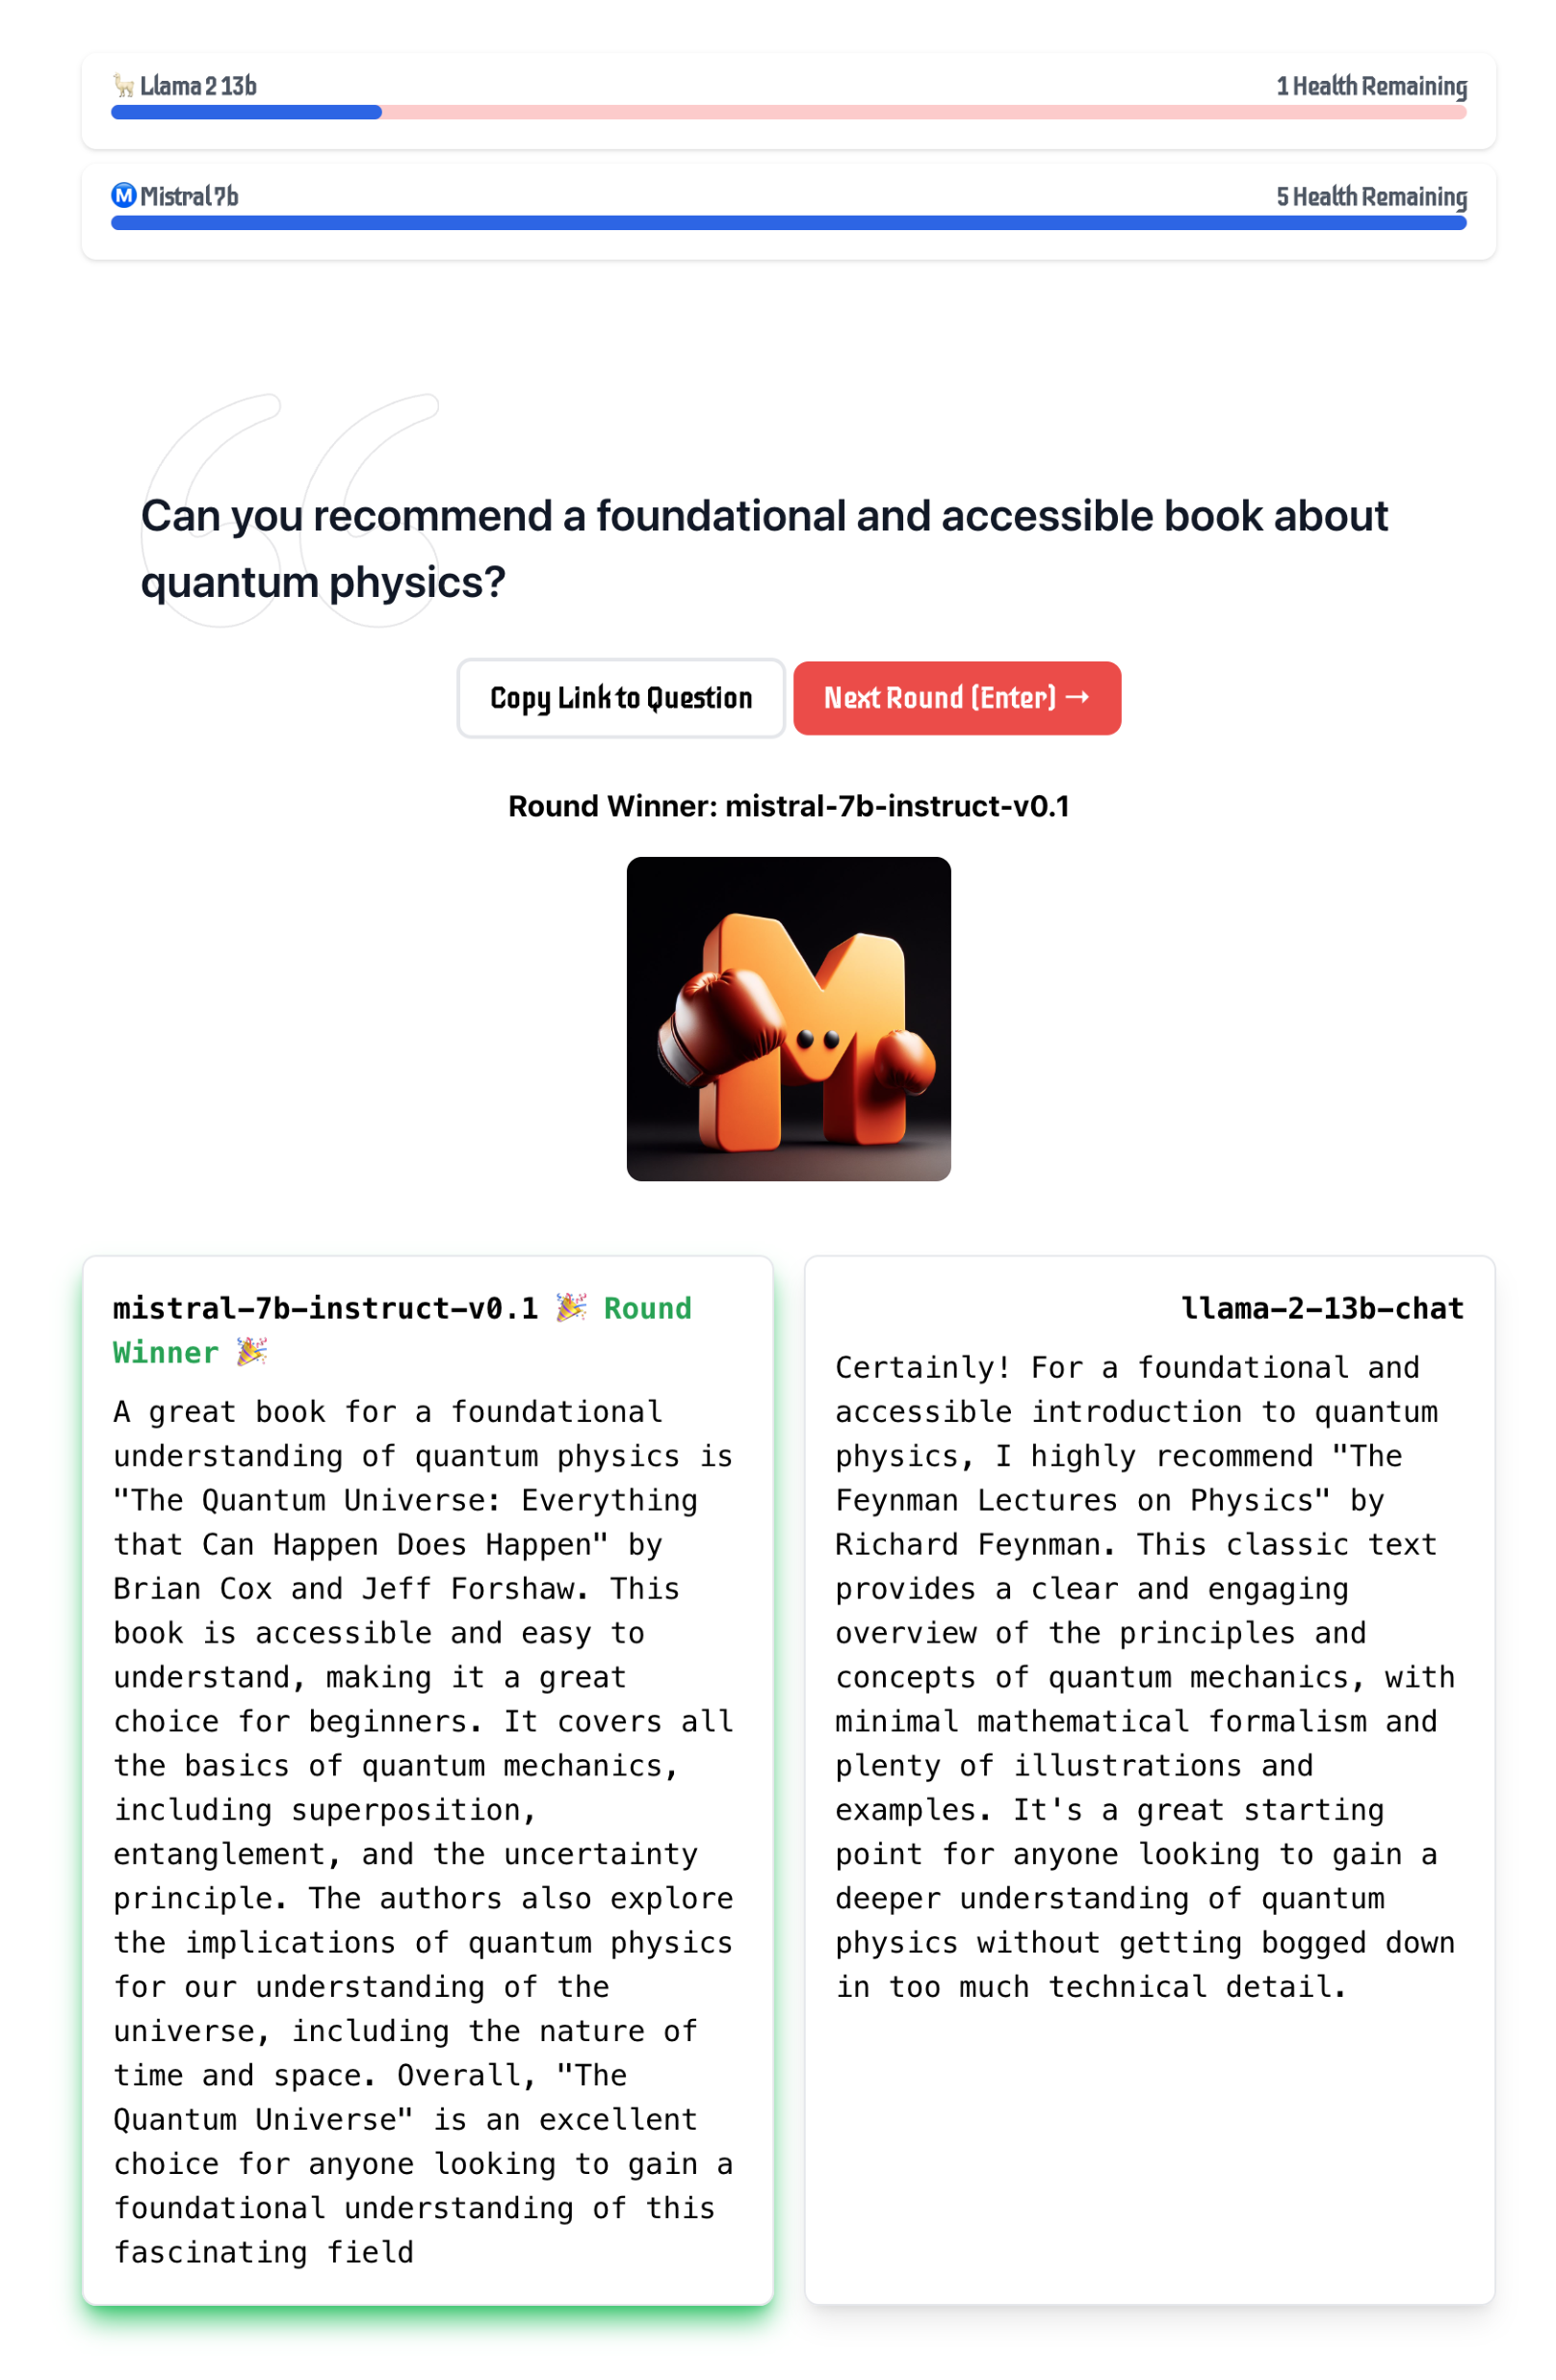
\includegraphics[width=0.5\textwidth]{fig6.png}
\caption{\bihead{\textbf{Human evaluation of Mistral 7B – Instruct vs Llama 2 13B – Chat Example.} An example of human evaluation from \texttt{llmboxing.com}. The question asks for recommendations of books in quantum physics. Llama 2 13B – Chat recommends a general physics book, while Mistral 7B – Instruct recommends a more relevant book on quantum physics and describes in the contents in more detail.}{\textbf{Mistral 7B – Instruct 与 Llama 2 13B – Chat 的人工评测示例。}这是来自 \texttt{llmboxing.com} 的一个人工评测示例。问题要求推荐量子物理方面的书籍。Llama 2 13B – Chat 推荐了一本普通物理学书籍，而 Mistral 7B – Instruct 推荐了一本更切题的量子物理书，并更详细地介绍了书中内容。\\
\textbf{图中文字：}顶部两条为“生命值”进度条——Llama 2 13b：剩余 1 点生命值（1 Health Remaining）；Mistral 7b：剩余 5 点生命值（5 Health Remaining）。问题：“你能推荐一本基础且通俗易懂的量子物理书吗？”按钮：Copy Link to Question＝复制问题链接；Next Round (Enter)＝下一轮（回车）。Round Winner: mistral-7b-instruct-v0.1＝本轮胜者：mistral-7b-instruct-v0.1。\\
左栏（mistral-7b-instruct-v0.1，本轮胜者）的回答：“要对量子物理建立基础性的理解，Brian Cox 和 Jeff Forshaw 合著的《量子宇宙：一切可能发生的都会发生》（The Quantum Universe: Everything that Can Happen Does Happen）是一本很好的书。这本书通俗易懂，非常适合初学者。它涵盖了量子力学的全部基础知识，包括叠加、纠缠和不确定性原理。作者还探讨了量子物理对我们理解宇宙的意义，包括时间与空间的本质。总之，对于任何希望对这一迷人领域建立基础性理解的人来说，《量子宇宙》都是绝佳的选择。”\\
右栏（llama-2-13b-chat）的回答：“当然！作为量子物理的基础入门读物，我强烈推荐 Richard Feynman 的《费曼物理学讲义》（The Feynman Lectures on Physics）。这部经典著作对量子力学的原理和概念做了清晰而引人入胜的概述，数学形式极少，并配有大量插图和示例。对于想要更深入地理解量子物理、又不想陷入过多技术细节的人来说，这是一个很好的起点。”}}
\label{fig:f6}
\end{figure}

\bisubsection{Content moderation with self-reflection}{基于自我反思的内容审核}
\label{sec:moderation}

\bipar{Mistral 7B – Instruct can be used as a content moderator: the model itself is able to accurately classify a user prompt or its generated answer as being either acceptable or falling into one of the following categories: Illegal activities such as terrorism, child abuse or fraud; Hateful, harassing or violent content such as discrimination, self-harm or bullying; Unqualified advice for instance in legal, medical or financial domains.}{Mistral 7B – Instruct 可以用作内容审核器（content moderator）：模型本身能够准确地把用户提示词或其生成的回答判定为“可接受”，或归入以下类别之一：违法活动，如恐怖主义、虐待儿童或欺诈；仇恨、骚扰或暴力内容，如歧视、自残或霸凌；不具备资质的建议，例如法律、医疗或金融领域的建议。}

\bipar{To do so, we designed a self-reflection prompt that makes Mistral 7B classify a prompt or a generated answer. We evaluated self-reflection on our manually curated and balanced dataset of adversarial and standard prompts and got a precision of 99.4\% for a recall of 95.6\% (considering acceptable prompts as positives).}{为此，我们设计了一个自我反思（self-reflection）提示词，让 Mistral 7B 对提示词或生成的回答进行分类。我们在一个人工整理、类别均衡、由对抗性提示词（adversarial prompts）和普通提示词组成的数据集上评估了自我反思的效果，在召回率（recall）为 95.6\% 时取得了 99.4\% 的精确率（precision）（以可接受的提示词作为正例）。}

\bipar{The use cases are vast, from moderating comments on social media or forums to brand monitoring on the internet. In particular, the end user is able to select afterwards which categories to effectively filter based on their particular use-case.}{其应用场景十分广泛，从审核社交媒体或论坛上的评论，到互联网上的品牌监测（brand monitoring），不一而足。特别地，终端用户可以根据自己的具体使用场景，事后选择需要实际过滤的类别。}

% =========================================================
\bisection{Conclusion}{结论}
\label{sec:conclusion}

\bipar{Our work on Mistral 7B demonstrates that language models may compress knowledge more than what was previously thought. This opens up interesting perspectives: the field has so far put the emphasis on scaling laws in 2 dimensions (directly associating model capabilities to training cost, as in \cite{ref14}); the problem is rather 3 dimensional (model capabilities, training cost, inference cost), and much remains to be explored to obtain the best performance with the smallest possible model.}{我们在 Mistral 7B 上的工作表明，语言模型对知识的压缩程度可能超出此前的认识。这带来了一些有趣的研究视角：迄今为止，该领域一直侧重于二维的缩放定律（scaling laws），即直接将模型能力与训练成本相关联（如文献~\cite{ref14}）；而这个问题实际上是三维的（模型能力、训练成本、推理成本），要用尽可能小的模型获得最佳性能，仍有大量问题有待探索。}

\section*{\bihead{Acknowledgements}{致谢}}

\bipar{We are grateful to CoreWeave for their 24/7 help in marshalling our cluster. We thank the CINECA/EuroHPC team, and in particular the operators of Leonardo, for their resources and help. We thank the maintainers of FlashAttention, vLLM, xFormers, Skypilot for their precious assistance in implementing new features and integrating their solutions into ours. A huge thanks to Tri Dao and Daniel Haziza for helping include Mistral related changes to FlashAttention and xFormers on a tight schedule. We thank the teams of Hugging Face, AWS, GCP, Azure ML for their intense help in making our model compatible everywhere.}{感谢 CoreWeave 全天候（24/7）协助我们调度和管理计算集群。感谢 CINECA/EuroHPC 团队，特别是 Leonardo 超级计算机的运维人员，为我们提供资源与帮助。感谢 FlashAttention、vLLM、xFormers 和 Skypilot 的维护者，在实现新功能以及将其方案集成到我们的系统中时给予的宝贵帮助。特别感谢 Tri Dao 和 Daniel Haziza 在紧张的时间安排下，帮助将 Mistral 的相关改动合入 FlashAttention 和 xFormers。感谢 Hugging Face、AWS、GCP 和 Azure ML 团队为使我们的模型在各个平台上兼容所提供的大力帮助。}

% =========================================================
\begin{thebibliography}{99}
\small
\bibitem{ref1} Joshua Ainslie, James Lee-Thorp, Michiel de Jong, Yury Zemlyanskiy, Federico Lebrón, and Sumit Sanghai. Gqa: Training generalized multi-query transformer models from multi-head checkpoints. arXiv preprint arXiv:2305.13245, 2023.
\bibitem{ref2} Jacob Austin, Augustus Odena, Maxwell Nye, Maarten Bosma, Henryk Michalewski, David Dohan, Ellen Jiang, Carrie Cai, Michael Terry, Quoc Le, et al. Program synthesis with large language models. arXiv preprint arXiv:2108.07732, 2021.
\bibitem{ref3} Iz Beltagy, Matthew E Peters, and Arman Cohan. Longformer: The long-document transformer. arXiv preprint arXiv:2004.05150, 2020.
\bibitem{ref4} Yonatan Bisk, Rowan Zellers, Jianfeng Gao, Yejin Choi, et al. Piqa: Reasoning about physical commonsense in natural language. In Proceedings of the AAAI conference on artificial intelligence, 2020.
\bibitem{ref5} Mark Chen, Jerry Tworek, Heewoo Jun, Qiming Yuan, Henrique Ponde de Oliveira Pinto, Jared Kaplan, Harri Edwards, Yuri Burda, Nicholas Joseph, Greg Brockman, et al. Evaluating large language models trained on code. arXiv preprint arXiv:2107.03374, 2021.
\bibitem{ref6} Rewon Child, Scott Gray, Alec Radford, and Ilya Sutskever. Generating long sequences with sparse transformers. arXiv preprint arXiv:1904.10509, 2019.
\bibitem{ref7} Eunsol Choi, He He, Mohit Iyyer, Mark Yatskar, Wen-tau Yih, Yejin Choi, Percy Liang, and Luke Zettlemoyer. Quac: Question answering in context. arXiv preprint arXiv:1808.07036, 2018.
\bibitem{ref8} Christopher Clark, Kenton Lee, Ming-Wei Chang, Tom Kwiatkowski, Michael Collins, and Kristina Toutanova. Boolq: Exploring the surprising difficulty of natural yes/no questions. arXiv preprint arXiv:1905.10044, 2019.
\bibitem{ref9} Peter Clark, Isaac Cowhey, Oren Etzioni, Tushar Khot, Ashish Sabharwal, Carissa Schoenick, and Oyvind Tafjord. Think you have solved question answering? try arc, the ai2 reasoning challenge. arXiv preprint arXiv:1803.05457, 2018.
\bibitem{ref10} Karl Cobbe, Vineet Kosaraju, Mohammad Bavarian, Mark Chen, Heewoo Jun, Lukasz Kaiser, Matthias Plappert, Jerry Tworek, Jacob Hilton, Reiichiro Nakano, et al. Training verifiers to solve math word problems. arXiv preprint arXiv:2110.14168, 2021.
\bibitem{ref11} Tri Dao, Daniel Y. Fu, Stefano Ermon, Atri Rudra, and Christopher Ré. FlashAttention: Fast and memory-efficient exact attention with IO-awareness. In Advances in Neural Information Processing Systems, 2022.
\bibitem{ref12} Dan Hendrycks, Collin Burns, Steven Basart, Andy Zou, Mantas Mazeika, Dawn Song, and Jacob Steinhardt. Measuring massive multitask language understanding. arXiv preprint arXiv:2009.03300, 2020.
\bibitem{ref13} Dan Hendrycks, Collin Burns, Saurav Kadavath, Akul Arora, Steven Basart, Eric Tang, Dawn Song, and Jacob Steinhardt. Measuring mathematical problem solving with the math dataset. arXiv preprint arXiv:2103.03874, 2021.
\bibitem{ref14} Jordan Hoffmann, Sebastian Borgeaud, Arthur Mensch, Elena Buchatskaya, Trevor Cai, Eliza Rutherford, Diego de Las Casas, Lisa Anne Hendricks, Johannes Welbl, Aidan Clark, Thomas Hennigan, Eric Noland, Katherine Millican, George van den Driessche, Bogdan Damoc, Aurelia Guy, Simon Osindero, Karén Simonyan, Erich Elsen, Oriol Vinyals, Jack Rae, and Laurent Sifre. An empirical analysis of compute-optimal large language model training. In Advances in Neural Information Processing Systems, volume 35, 2022.
\bibitem{ref15} Mandar Joshi, Eunsol Choi, Daniel S Weld, and Luke Zettlemoyer. Triviaqa: A large scale distantly supervised challenge dataset for reading comprehension. arXiv preprint arXiv:1705.03551, 2017.
\bibitem{ref16} Tom Kwiatkowski, Jennimaria Palomaki, Olivia Redfield, Michael Collins, Ankur Parikh, Chris Alberti, Danielle Epstein, Illia Polosukhin, Jacob Devlin, Kenton Lee, et al. Natural questions: a benchmark for question answering research. Transactions of the Association for Computational Linguistics, 7:453--466, 2019.
\bibitem{ref17} Woosuk Kwon, Zhuohan Li, Siyuan Zhuang, Ying Sheng, Lianmin Zheng, Cody Hao Yu, Joseph E. Gonzalez, Hao Zhang, and Ion Stoica. Efficient memory management for large language model serving with pagedattention. In Proceedings of the ACM SIGOPS 29th Symposium on Operating Systems Principles, 2023.
\bibitem{ref18} Benjamin Lefaudeux, Francisco Massa, Diana Liskovich, Wenhan Xiong, Vittorio Caggiano, Sean Naren, Min Xu, Jieru Hu, Marta Tintore, Susan Zhang, Patrick Labatut, and Daniel Haziza. xformers: A modular and hackable transformer modelling library. \url{https://github.com/facebookresearch/xformers}, 2022.
\bibitem{ref19} Todor Mihaylov, Peter Clark, Tushar Khot, and Ashish Sabharwal. Can a suit of armor conduct electricity? a new dataset for open book question answering. arXiv preprint arXiv:1809.02789, 2018.
\bibitem{ref20} Baptiste Rozière, Jonas Gehring, Fabian Gloeckle, Sten Sootla, Itai Gat, Xiaoqing Ellen Tan, Yossi Adi, Jingyu Liu, Tal Remez, Jérémy Rapin, et al. Code llama: Open foundation models for code. arXiv preprint arXiv:2308.12950, 2023.
\bibitem{ref21} Keisuke Sakaguchi, Ronan Le Bras, Chandra Bhagavatula, and Yejin Choi. Winogrande: An adversarial winograd schema challenge at scale. Communications of the ACM, 64(9):99--106, 2021.
\bibitem{ref22} Maarten Sap, Hannah Rashkin, Derek Chen, Ronan LeBras, and Yejin Choi. Socialiqa: Commonsense reasoning about social interactions. arXiv preprint arXiv:1904.09728, 2019.
\bibitem{ref23} Mirac Suzgun, Nathan Scales, Nathanael Schärli, Sebastian Gehrmann, Yi Tay, Hyung Won Chung, Aakanksha Chowdhery, Quoc V Le, Ed H Chi, Denny Zhou, and Jason Wei. Challenging big-bench tasks and whether chain-of-thought can solve them. arXiv preprint arXiv:2210.09261, 2022.
\bibitem{ref24} Alon Talmor, Jonathan Herzig, Nicholas Lourie, and Jonathan Berant. Commonsenseqa: A question answering challenge targeting commonsense knowledge. arXiv preprint arXiv:1811.00937, 2018.
\bibitem{ref25} Hugo Touvron, Thibaut Lavril, Gautier Izacard, Xavier Martinet, Marie-Anne Lachaux, Timothée Lacroix, Baptiste Rozière, Naman Goyal, Eric Hambro, Faisal Azhar, et al. Llama: Open and efficient foundation language models. arXiv preprint arXiv:2302.13971, 2023.
\bibitem{ref26} Hugo Touvron, Louis Martin, Kevin Stone, Peter Albert, Amjad Almahairi, Yasmine Babaei, Nikolay Bashlykov, Soumya Batra, Prajjwal Bhargava, Shruti Bhosale, et al. Llama 2: Open foundation and fine-tuned chat models. arXiv preprint arXiv:2307.09288, 2023.
\bibitem{ref27} Ashish Vaswani, Noam Shazeer, Niki Parmar, Jakob Uszkoreit, Llion Jones, Aidan N Gomez, Łukasz Kaiser, and Illia Polosukhin. Attention is all you need. Advances in neural information processing systems, 30, 2017.
\bibitem{ref28} Rowan Zellers, Ari Holtzman, Yonatan Bisk, Ali Farhadi, and Yejin Choi. Hellaswag: Can a machine really finish your sentence? arXiv preprint arXiv:1905.07830, 2019.
\bibitem{ref29} Wanjun Zhong, Ruixiang Cui, Yiduo Guo, Yaobo Liang, Shuai Lu, Yanlin Wang, Amin Saied, Weizhu Chen, and Nan Duan. Agieval: A human-centric benchmark for evaluating foundation models. arXiv preprint arXiv:2304.06364, 2023.
\end{thebibliography}

\end{document}

